\documentclass[10pt, conference, compsocconf]{IEEEtran}
\usepackage{url}

\usepackage{amsmath,amssymb}
\usepackage{graphicx}
\usepackage{color}

% correct bad hyphenation here
\hyphenation{}


\begin{document}
%
% paper title
% can use linebreaks \\ within to get better formatting as desired
\title{Towards Minimizing the Required Bandwidth for Mobile Web Browsing}

% author names and affiliations
% use a multiple column layout for up to two different
% affiliations

\author{\IEEEauthorblockN{Madhuvanthi Jayakumar, Marcela Melara, and Nayden Nedev}
\IEEEauthorblockA{Princeton University\\
\{jmadhu, melara, nnedev\}@cs.princeton.edu}}

% make the title area
\maketitle

\begin{abstract}
%The number of smartphones has been increasing in a very fast pace over the last several 
%years. With this speed, it is quite likely that they will dominate the market in the very 
%near future. As a result, the amount of mobile Web traffic now takes a serious portion of 
%the total amount of Internet traffic. Moreover, it is expected to grow exponentially with 
%every subsequent year. These facts put new challenges in the ways mobile networks are designed 
%and built. New methods for alleviation of the amount of transmitted mobile web traffic data
%should be found. 

%In this paper, we propose a novel technique for reducing the needed bandwidth for mobile Web 
%browsing. It automatically identifies redundancies in mobile Web sites data and cuts the number
%of transimitted bytes. We leverage partitioning of website data into chunks and fingerprinting them
%for efficient retrieval from a cache. The only addition to the network that our method requires 
%is a dedicated proxy server which serves as a cache. We implement our techniques in a sophisticated 
%simulator and evaluate their effectiveness on a number of popular websites. Our empirical results 
%show that, with an appropriate tuning of all system components, the needed bandwidth can be reduced 
%to less than 10\% in some cases.

The number of smartphones has been increasing at a very fast pace over the last several 
years. At this rate, it is quite likely that mobile web traffic will take a serious portion of the global Internet traffic in the very near future. However, the improvement of mobile web access technology has been known to lag behind the current growth: we face issues such as limited bandwidth and computational power and high latency. Additionally, users have financial incentives to use their limited data plan effectively.
These facts motivate new ways of designing and building mobile web access technologies and networks. Specifically, new methods for reducing mobile web traffic and for utilizing the mobile computational and network resources more efficiently should be found.

In this paper, we propose a novel technique for reducing the needed bandwidth for mobile web browsing. It automatically identifies redundancies in mobile website data to reduce the number of transmitted bytes. We leverage the standard deduplication techniques of partitioning website data into chunks and fingerprinting them
for redundancy detection and efficient retrieval from a cache. The only additions to the current mobile browsing framework that our method requires is a dedicated proxy server and the installation of a mobile proxy-client. We implement our techniques in a sophisticated  simulator and evaluate their effectiveness on a number of popular websites. Our empirical results show that, with an appropriate tuning of all system components, the needed bandwidth can be consistently reduced to less than 20\% in most cases.
\end{abstract}

%\begin{IEEEkeywords}
%component; formatting; style; styling;
%\end{IEEEkeywords}

% For peer review papers, you can put extra information on the cover
% page as needed:
% \ifCLASSOPTIONpeerreview
% \begin{center} \bfseries EDICS Category: 3-BBND \end{center}
% \fi
%
% For peerreview papers, this IEEEtran command inserts a page break and
% creates the second title. It will be ignored for other modes.
\IEEEpeerreviewmaketitle

%\category{}{}{}

\section{Introduction}
% Motivation
As of the beginning of 2013, global mobile traffic represented roughly 13\% of internet traffic \cite{?}. In 2009, this number was just 1\%, moved up 
to 4\% in 2010, and is expected to grow exponentially over the next X years \cite{?}. Of the 5 billion mobile phones in the world, only a fifth are 
smartphones \cite{?}. The user base of smartphone is expected to expand by about 42\% a year, and with that grows the mobile web traffic \cite{?}. The 
issue we face is that mobile networks in North America are already running at 80\% of capacity and 36\% of base stations are facing capacity constraints 
\textbf{[what does ``capacity constraints" mean]} \cite{?}. Globally, the ubiquitous appearance of mobile devices with the rise of cheap smartphones and 
tablets in developing countries such as Africa and India is creating a demand for available and affortable bandwidth as well. In addition to the computational 
barriers, the data limits posed on mobile carrier data plans and data overage charges are an incentive for users to utilize their available data effectively. 

%Intro to Previous Work
The growth in demand of mobile network bandwidth in conjunction with the financial incentives of smartphone users motivates new and innovative techniques 
to reduce mobile network traffic, and to use mobile bandwidth more efficiently. One property of web data pertaining especially to content viewed through a 
web browser is of particular use for increasing the efficiency of mobile bandwidth utilization: Data redundancy. Specific pages and sites have the tendency 
to change little over time. Thus, when making a new request for some specific web content, the response will often contain a small number of modifications, 
but will, for the most part, be identical to a previously requested version of this content. While there has been previous work in this area analyzing redundant 
desktop browser data \cite{?}, there has been minimal study of data redundancy in the area of mobile browsing.

% Nayden: More motivation needed here

% Our Method 
% Nayden: This is too long for introduction. I don't think we need so many details. They should go to the design or implementation and here we should
% mention only basic things.
We present a technique which leverages these data redundancies to improve the bandwith utilization efficiency of mobile browsers. We use data deduplication 
techniques to find the content a requesting mobile client actually needs, avoiding the transfer of redundant data. By focusing purely on redundancies in web 
page content, our mechanism helps reduce the number of bytes sent across the network, thereby reducing the required bandwidth. We integrate our technique into 
the data processing phase of browsing, i.e. the phase between the initial request for a page and the rendering of the requested page. More specifically, we add 
the following three steps: (1) Data Chunking which partitions incoming web content into fixed-size data chunks, (2) Fingerprinting which uses fingerprinting 
techniques to create a unique encoding of each unique data chunk, and (3) Caching which adds a layer on top of the web cache to only store unique chunks of data. 
We use a proxy server to perform the computationally intensive steps (1) and (2) to minimize the additional strain on the limited computational resources of mobile 
devices.

%Other Methods --> Moved to discussion

% Purpose
Our technique allows us to analyze redundancies across and within websites and to calculate the amount of potential bandwidth savings that can be obtained through data deduplication. As part of our analysis, we test various data chunk and cache sizes with the aim of finding the optimal parameter settings for our technique. We have built a simulator to perform these analyses using use two datasets, one obtained by capturing HTTP response packets through the packet analysis tool Wireshark and the other obtained through telnet requests. We also study various implementations of cache eviction algorithms to determine the optimal choice for our technique. Additionally, we have implemented a proof-of-concept networked mobile client simulator and basic proxy server showing that our technique does not require changes to web server configurations, and does not alter the mobile browsing experience, making this a viable enhancement to mobile browsers benefitting mobile users.

The rest of this paper is organized as follows. We discuss the previous work done on the problem in Section~\ref{sec:rel_work}. We describe the basic design of the 
system that we built in Section~\ref{sec:sys_design} and ~\ref{sec:protocol}. Details about our implementation are presented in Section~\ref{sec:implementation} 
and results of experimental evaluation in Section~\ref{sec:eval}. We discuss the results of the evaluation that we performed in Section~\ref{sec:discussion}, give 
some directions for potential future work and conclude in Section~\ref{sec:conclusion}.

\section{Previous Work}\label{sec:rel_work}
Some work has been done in trying to reduce bandwidth in wide-area networks. Ihm \textit{et al.}~\cite{wanax} present 
a system for reducing bandwidth in wide-area networks for efficient Internet usage in developing countries. Their 
technique is similar to the one used in this work, \textit{e.g.} chunking of the stream of data and Rabin fingerprinting 
of the resulting chunks. However, they are assuming large and small  

Ihm and Pai~\cite{modern_web_traffic} perform a thorough and deep analysis of Web traffic logs that have been collected 
over five-years period. They find many interesting facts about connection speed of today's Web users, NAT usage, content type
of the traffic and the traffic share of different types of Web sites. Moreover, they find that there is a fair amount 
of redundancy in the Web traffic and discuss different approaches for reducing the amount of this redundancy.

Qian \textit{et al.}~\cite{web_caching}

\section{System Design}
\label{sec:sys_design}
At the core of our technique lies the ad hoc system and protocol we integrate into the existing mobile browsing framework in place today. This system is comprised of a specially configured proxy server, a per-device mobile proxy client, each of which manages specific tasks in our deduplication mechanism. Our protocol specifies the data exchanged between these two components. We integrate our system into the data processing phase of browsing, i.e. the phase between the initial request for a page and the rendering of the requested page.

In our system, the proxy server and mobile proxy clients are logically located between the mobile browser and the Web, managing requests for web pages coming from the browser and engaging in the bandwidth reduction protocol. Most of the computation for our deduplication mechanism occurs on the proxy server so as to minimize the additional strain on the limited computational resources of mobile devices, while the mobile proxy client supplies the proxy server with relevant information it needs to find data redundancies. 

For our deduplication mechnism, we borrow several techniques proven useful for identifying similarities between files and data streams. In particular, we use the following two: 
\begin{enumerate}
\item Chunking: Partition incoming web content into data chunks.
\item Fingerprinting: Create a unique encoding for each unique data chunk.
\end{enumerate}
We explore two chunking techniques and use the implementation for Rabin Fingerprinting given by Broder \cite{broder}. 

In addition, our mechanism requires special caches, one on the proxy server, and one on the mobile proxy client to store unique chunks of data. The client cache replaces the built-in browser web cache. We assume multiple mobile devices connecting to the proxy server and making distinct, un-correlated requests such that our mechanism does not attempt to synchronize the proxy server and client caches.

\subsection{Chunking}
\label{sec:chunking}
\subsubsection{Fixed-Size Chunking}

\subsubsection{Sliding Window Chunking}
The second chunking technique we explore is what we call sliding window chunking, a technique originally presented by Manber in order to find similarities between different files \cite{Manber}. As opposed to partitioning files and streams of data into fixed-size chunks, which are inflexible to file and packet content boundaries, this method allows us to adapt chunk sizes based on the actual contents of the file or packet stream. This is done by choosing a fixed-size window which we slide across the entire contents of a web page, and fingerprinting each region until some number of low-order bits of the fingerprint are all 0. Once this occurs, we have found a breakpoint and the chunk boundary is set to the end of this special window. 

We compute our sliding window chunks based on the equations and parameters presented in \cite{spring} and combine them with the enhancements used in the LBFS content-based breakpoint chunking scheme \cite{lbfs}. Thus, not only do we specify a window size $\beta$ and breakpoint fingerprint value with $\gamma$ zeros in the low-order bits, we also specify a minimum and maximum chunk size. 

The purpose of chosing this scheme over the fixed-size chunking scheme is rather straight-forward. Since the chunks are chosen based on content rather than on position in the web page, minor changes will not affect surrounding chunks. In contrast, any minor change to a web page will probably shift a large number fixed-size chunks by some amount causing changes to a large number of fingerprints, which in turn leads to an overall decrease in redundancy detection. Unlike Manber, and Spring and Wetherall, who use this chunking scheme to fingerprint every possible region in a file or packet and then choose a specific subset of these fingerprints to find redundant data \cite{manber,spring}, we use the same approach as LBFS, i.e. to use these scheme merely for finer-grained chunking of the data and determine redundancies using additional hashing or fingerprinting once the chunks have been found. We discuss Rabin fingerprinting for the purposes of finding redundant data chunks in Section \ref{sec:fingerprinting}. 



\subsection{Data Fingerprinting}
\label{sec:fingerprinting}
Data fingerprinting is the second deduplication technique we use in our bandwidth reduction mechanism. In general, a fingerprinting function is similar to a hash function in that it is also a one-way function which maps an arbitrarily large input to a fixed-size number, and each unique input has a unique fingerprint value. However, unlike an conventional hash function, this fingerprinting function can be decomposed for the incremental computation of a fingerprint. This is done by representing the input as a polynomial modulo a pre-determined irreducible polynomial \cite{rabin,lbfs}.

Our use of fingerprinting is two-fold: (1) To generate the sliding window chunks, and (2) to generate fingerprints as identifiers for unique chunks. We exploit the fact that any size chunk maps to a fixed-size fingerprint, which is much more efficient to transfer across the network than the entire data chunk. As we discuss in more detail in Section \ref{sec:protocol}, our mechanism requires the transmission of two rounds of fingerprints for data redundancy detection but the total bandwidth savings of our system outweigh these added overhead and bandwidth requirements of these two additional transmissions (see Section \ref{sec:eval}).
\subsection{Caching}
\label{sec:caching}
Another main component of our system are two caches - one in the proxy server and one in the 
mobile client. Each of them maintains a mapping between fingerprints and the chunks that they
represent. Each chunk is being fingerprinted and then requested from either of the caches. There
are no specific restrictions to the internal representation of the caches and their size, \textit{i.e.}
how they work internally is irrelevant to the way the other components of the system work.

%\subsection{Bandwidth Reduction Protocol}
\label{sec:protocol}
The second major part of our technique is the reduction protocol between the mobile device and the proxy server. It brings together all the components described in Section \ref{sec:sys_design}. Every time a new page is requested by the mobile browser, the following protocol is performed:
\begin{enumerate}
\item Mobile device sends an HTTP request to the proxy server.
\item Proxy server relays this request to the proper web server.
\item Proxy server performs chunking and fingerprinting of the chunks for all the received web content. It sends all the fingerprints to the mobile device.
\item Mobile device checks its cache for the fingerprints, and creates a list of those it needs. It sends this list to the proxy server.
\item Proxy server creates a list of the needed chunks according to the received needed fingerprints. It sends this list back to the mobile device.
\item Mobile device reconstructs the entire requested page from its cache contents and the received list of needed chunks.
\end{enumerate}







\section{Simulator Implementation}
\label{sec:implementation}
We implemented two versions of a simulator of our system: 
\begin{enumerate}
\item An offline simulator, which uses data collected and stored during a mobile browsing session, and input into the simulator offline, and
\item A networked simulator, which simulates a basic incarnation of our system in real-time.
\end{enumerate}
Both simulators are written in Java, and use five helper interfaces and classes each one representing a component of the system, in addition to the proxy server and mobile device classes. In particular, we use two helper interfaces: \texttt{ICache} and \texttt{IProcessor}. \texttt{ICache} allows for different implementations of caches supporting various eviction algorithms. \texttt{IProcessor} allows creating different cache processors. A cache processor is an entity which interfaces a device and its web cache, with its most important task to process incoming web content based on the device's cache contents. While both of our simulators use a single implementation of \texttt{IProcessor} called \texttt{SimpleProcessor}, which manages web content caching, and measures the cache hit-rate and miss-rate, we have multiple implementations of \texttt{ICache}, which we address later in this section. 

The three helper classes we use are \texttt{Chunk}, \texttt{Chunking} and \texttt{Fingerprinting}. The \texttt{Chunk} class defines a chunk with a given size in number of bytes and the data. \texttt{Chunking} is the facility which generates all the data chunks for a given input, either an input file containing web page data or a data stream of online web data. The \texttt{Fingerprinting} class is a wrapper for the Java \emph{rabinhash} library \cite{rabinhash}, and uses 32-bit fingerprints of a given chunk \cite{rabin_api}.

Finally, we created the \texttt{ISimulator} interface to build different kinds of simulators. Our offline version uses one or more \texttt{Mobile} devices and a \texttt{ProxyServer} to implement the simulation of our reduction protocol described in Section \ref{sec:protocol}. The networked simulator uses the networked counterparts of these two components.

Figure \ref{fig:class_diagram} summarizes our implementation software in its entirety\footnote{Blue lines denote aggregation with the cache and are merely for legibility purposes.}.

\begin{figure*}[ht] \centering 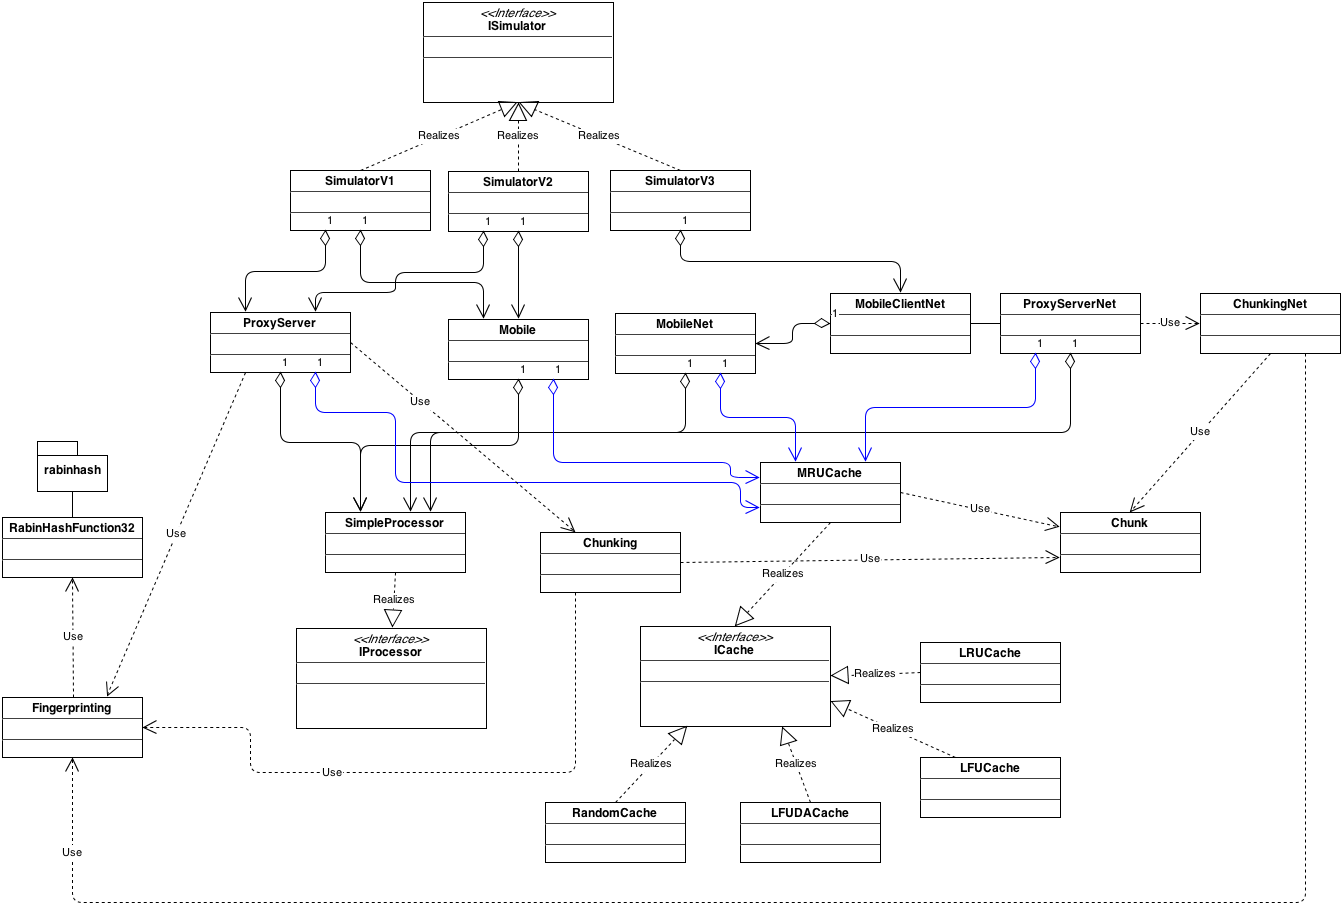
\includegraphics[scale=0.3]{images/class_diagram.png}
\caption{Implementation Software Class Hierarchy.}
\label{fig:class_diagram}
\end{figure*}

\subsection{Offline Simulator}
\subsection{Networked Simulator}
\label{sec:netsim}
The networked simulator consists of the proxy server (\texttt{ProxyServerNet}) and the mobile client simulator (\texttt{SimulatorV3} run on a departmental Ubuntu server), which is a wrapper for the networked mobile proxy-client (\texttt{MobileClientNet}) and is capable of performing several rounds of requests to the proxy server in real-time. It does so by prompting the user to manually enter the next web page URL she wishes to visit, simulating web browser interactions (see Figure \ref{fig:mobsim_ui} for an example of the user interface of our mobile client). The simulator architecture can be seen in Figure \ref{fig:netsim_arch}. 

\begin{figure*}[ht] 
\centering 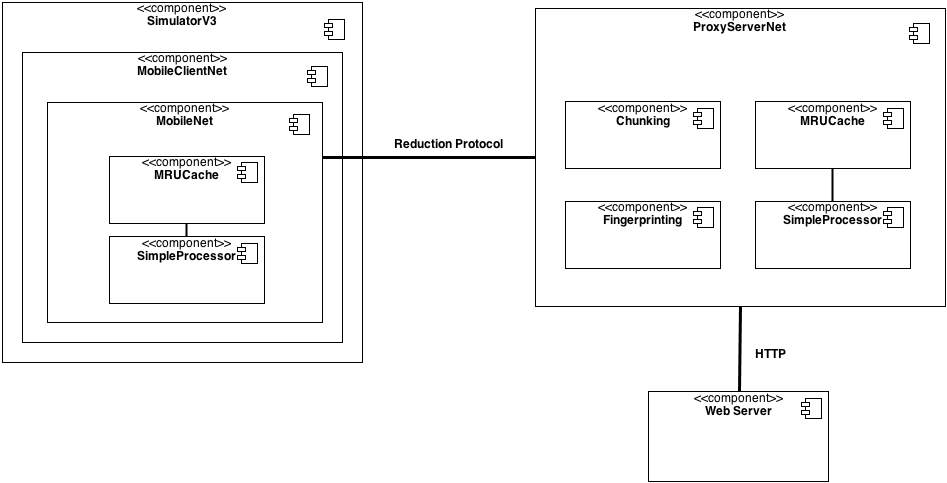
\includegraphics[scale=0.40]{images/component_diagram.png}
\caption{Networked Simulator Runtime Interactions.}
\label{fig:netsim_arch}
\end{figure*}

\begin{figure}[h] 
\centering 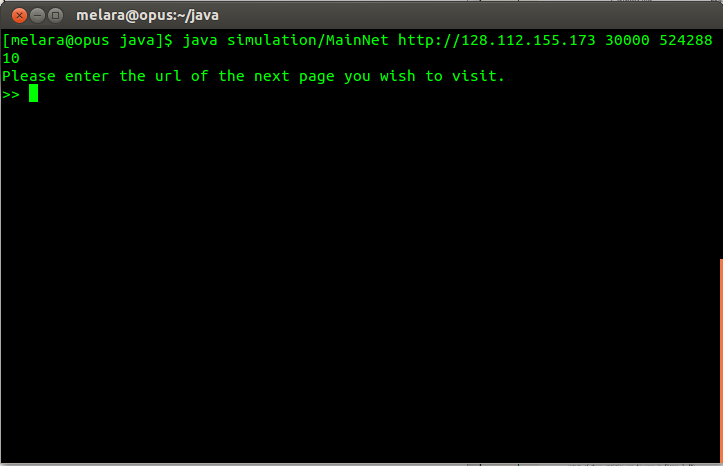
\includegraphics[scale=0.40]{images/mobilesim_ui.png}
\caption{The User Interface of our Mobile Client Simulator.}
\label{fig:mobsim_ui}
\end{figure}

In more detail, the networked simulator implements our reduction protocol as follows. First, the mobile proxy-client opens a socket to the proxy server, which is listening for connections at a user-specified port. The mobile proxy-client sends a simplified HTTP request of the format \emph{GET $<$url$>$ HTTP/1.1} to the proxy server. It then formulates a proper HTTP request, including the User-Agent string of a mobile device\footnote{We use the Samsung Galaxy SII as our model mobile device across all our implementations and experiments.} to ensure that it receives the mobile version of the requested web page from the hosting web server. Once the proxy has received the content of the requested page from the appropriate web server, it engages in the bandwidth reduction protocol\footnote{Minor changes were made to the chunking facility as well as the mobile device definition to support networking.} with the mobile proxy-client, exchanging the relevant information via the network. At the end, the mobile proxy-client reconstructs the content data of the received web page into an HTML file, which can then be viewed in any web browser. After the proxy has served the mobile client's request, the client is able to make a new request and repeat this process.

We found that, while simulating mobile browsing, for one not using an actual mobile phone, and for another not using a web browser program of any sort, is not realistic, our networked simulator is a good first proof-of-concept prototype showing that our reduction protocol is viable. In our experimental evaluation, we argue that it reduces the required bandwidth compared to the currently required mobile browsing bandwidth.

In the end, we would like to discuss some caveats of our networked simulator. First, as our mobile client simulator does not have the capabilities of a web browser and it receives preprocessed data from the proxy server, it cannot automatically handle HTTP responses indicating page redirects (i.e. server response code $301$, for example). Thus, our proxy server handles HTTP responses with the server response codes $200$ and $40X$\footnote{$200$ means granted normally, $40X$ response codes indicate a form of client-side error such as malformed requests but return HTML-format content with this information.} since the web server returns HTML content with these responses. An additional consequence of the fact that our mobile client is not browser-like is that it must create a local copy of each retrieved web page. Although the content of the web page is reconstructed correctly, since many links within web pages point to relative paths, the retrieved web pages are often rendered incorrectly in the local web browser as it cannot find cascading stylesheets (CSS) and embedded images on the local disk. We propose how to solve these issues in our discussion on future work.

\subsection{Using Different Caching Algorithms}

\section{Experimental Evaluation}
\label{sec:eval}

We obtained results through a process of collecting offline data, and modifying our simulator to output information about the data being processed. 
Mainly, we observed how changes in parameters affected the miss rate as well as the number of bytes transferred between the proxy and mobile device.

In order to run our experiments, we first collected offline data. 
Over the course of four days, we issued telnet GET requests to various webpages (both desktop and mobile versions) in the morning, afternoon and evening. 
The frequency with which we made these GET requests were for the purpose of reflecting browsing patterns, and it would give us information about the change in the content of a webpage over the course of a day and over the course of multiple days. 
We stored each response in a different file and then processed the data to obtain the byte stream version of the html pages. 
Using this byte stream, we ran several experiments that gave us insight into data redundancy within webpages.

Figure shows the distinctions between mobile web content and desktop web content. 
Many web servers today structure their webpages differently depending on the user-agent they're serving to increase the speed with which the webpages load, to provide better service with respect to UI and various other reasons. 
Therefore, mobile pages are inherently different from desktop browsers and thereby require its own analysis. 
Figure shows that the mobile version of cnn.com is only about a fifth of the size of the desktop version. 
The bytes transferred for the unchunked protocol shows that the size of the webpage remains relatively constant, and that the entire webpage has to be reloaded from the server for each request since the content is no longer "fresh". 
The bytes tranferred with the chunked protocol shows that the amount of redundancy that is eliminated in both mobile and desktop websites is proportional to the size of the web page. 
It also provides insight into exactly where our protocol performs well, and where the overhead of the protocol takes away from the benefits achieved from chunking. 
We see that on the first visit, the amount of bytes that needs to be transferred is almost twice the size of the actual content. 
This inefficiency comes from the fact that we're using chunk size of ten bytes. 
During the first visit to cnn.com, when there is no base copy of the webpage, the fingerprints representing the entire webpage need to be sent back and forth creating an inefficiency. 
However, once there is a base copy in the cache, the overhead decreases substantially. 
We can see from the graph that by the 12th visit, we are only transferring half the number of bytes as we would need to reload the entire webpage. 

The use of chunk size of 10 bytes means that each redundant chunk saves 6 bytes because of the 4 bytes of fingerprint needed to represent that chunk. 
This led us to explore different chunksizes to find the ideal chunk size that takes into consideration the tradeoff between having a low cache miss rate and having a fingerprint map to a bigger chunk. 
This is innately tied to the size of the content. Figure shows the relationship between \% of web content that is needed (based on cache miss rate) and chunk size based on a series of visits to cnn.com. 
The first visit is not shown since the cache is empty and so 100\% of the content needs to be transferred for all chunk sizes. 
The graph shows data from the second day, assuming cache has already been filled with data from the first visit. 
It is clear from this graph that if we use smaller chunk sizes, the percent of content that needs to be sent decreases. 
The steeper line for chunk 5 when compared to chunk 45 shows that as the number of visits increase, the overlap of smaller chunk sizes increases faster.
However, it means that each fingerprint maps to a smaller chunk and so more fingerprints are needed to represent the small amount of data that needs to be transferred and fewer fingerprints are needed to represent a large amount of data. 
In figure we can see that as the chunk size increased, the miss rate also increased as expected, but the bytes transferred actually decreased. 
This is because if the chunk size is small it gets expensive for the mobile device to communicate which chunks it needs. 
At this point, the ideal chunk size depends on the size of content that needs to be transferred as opposed to percentage.

The next two graphs show what happens when we visisted three websites three times a day for four days to simulate "mobile browsing". 
Figure shows that on the the first visit, the cache is empty and 100\% of the traffic needs to be transferred. 
For the second website, almost all of it needs to be transferred (~90\%) because of lack of overlap with the first website. 
On the third, the proportion decreases further but a majority of the page still needs to be transferred. 
After this point, we have the base page for all three websites in our cache and only the differences need to be transferred from the proxy, so the proportion of content that needs to be transferred stays below 20\% by the sixth url request. 
This figure calculates the proportion of content that needs to be transferred based on the cache miss rate but does not take into account the additional bytes that have to be transferred due to fingerprints.

Figure shows the total number of bytes that were transferred for the 32 requests. 
We assume that no response is identical to a previous response. 
This means that without chunking, the full webpage has to be reloaded for each request, leading to the linearly increasing number of bytes we see in the graph. 
With chunking however, we see that past the first few requests in which the effects of the overhead are heavy, the number of total bytes transferred rises gradually, and the gap between the bytes transferred grows with the number of requests.


\begin{figure}[h] 
\centering 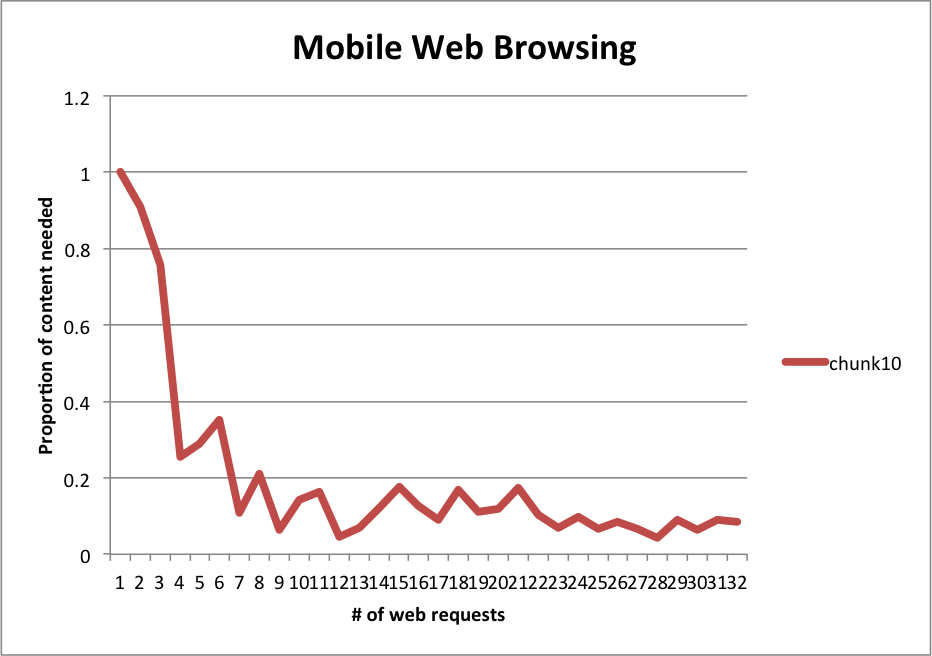
\includegraphics[scale=0.40]{images/browsing.png}
\caption{Mobile Web Browsing. The data was gathered by visiting cnn.com, nytimes.com and economist.com in an alternating basis three times a day over four days. This graph shows that the if the 'base' content of each webpage is in the cache, then less than 20\% of the content is generally new. The first three requests show that there is some, but not a lot of redundancy between webpages.}
\label{fig:mobsim_ui}
\end{figure}

\begin{figure}[h] 
\centering 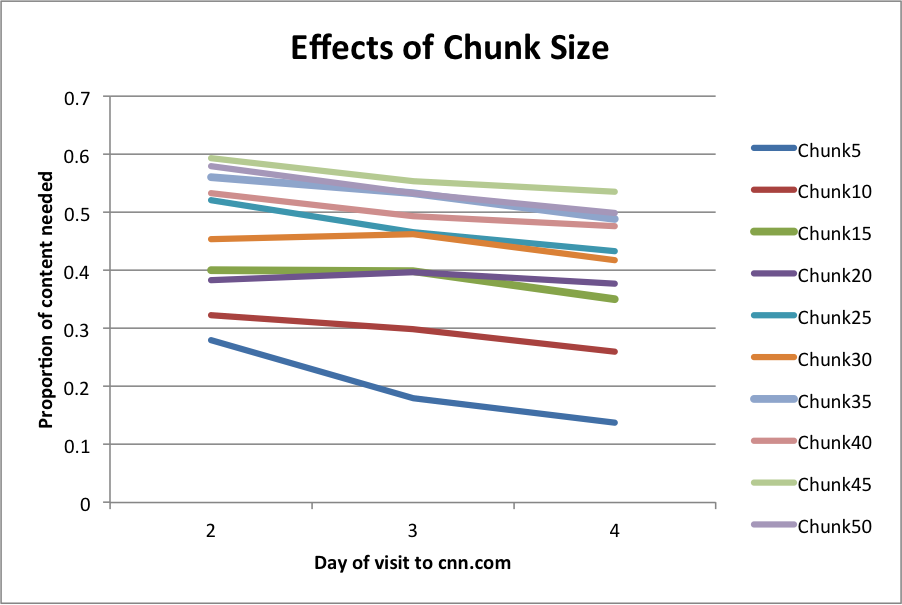
\includegraphics[scale=0.40]{images/chunksize.png}
\caption{Effects of Chunk Size on portion of content needed obtained through visit to cnn once a day for four days. Day 1 is not shown since the cache is empty so the contents of the entire webpage needs to be transferred.}
\label{fig:mobsim_ui}
\end{figure}

\begin{figure}[h] 
\centering 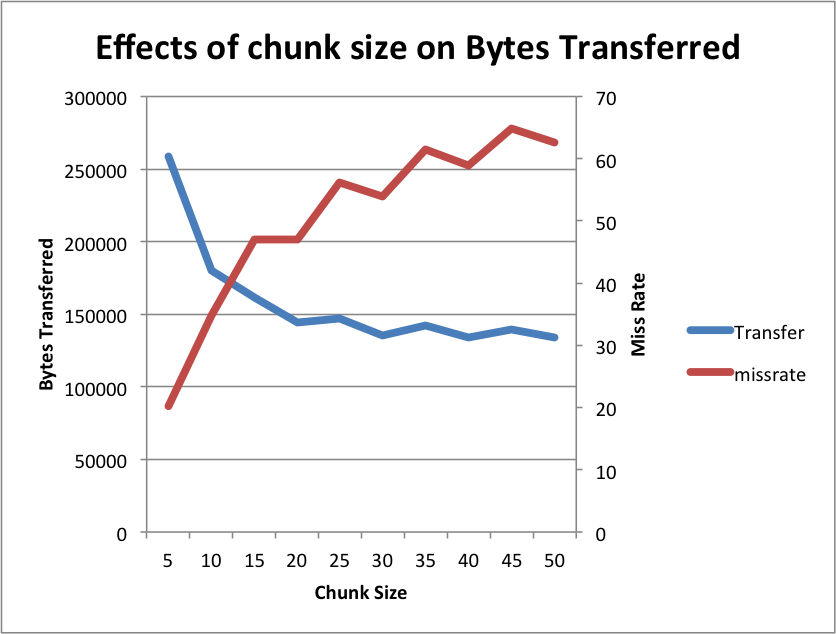
\includegraphics[scale=0.40]{images/chunksize2.png}
\caption{Effects of chunk size on Bytes Transferred. This graph takes into account the effects of the extra bytes that need to be transferred to account for the fingerprints that needs to be transferred to represent redndant chunks.}
\label{fig:mobsim_ui}
\end{figure}

\begin{figure}[h] 
\centering 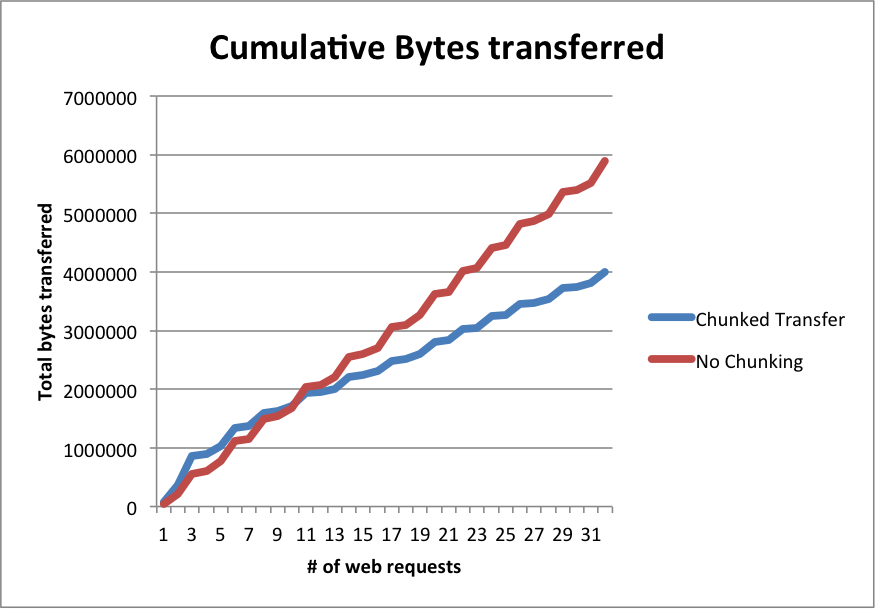
\includegraphics[scale=0.40]{images/cumulbrowsing.png}
\caption{Cumulative bytes transferred during browsing. This shows the bandwidth savings obtained from chunking.}
\label{fig:mobsim_ui}
\end{figure}

\begin{figure}[h] 
\centering 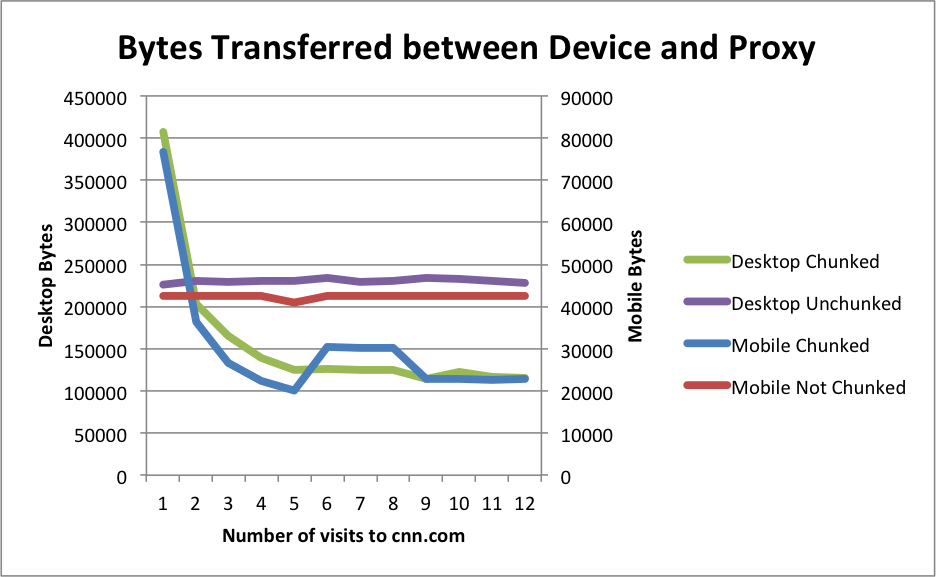
\includegraphics[scale=0.40]{images/desktopmobile.png}
\caption{Desktop vs Mobile Browser page differences.}
\label{fig:mobsim_ui}
\end{figure}


\section{Discussion}
Other techniques that have been used to reduce bandwidth are data compression \cite{?} and partial responses \cite{?}. For our purposes, we use data deduplication because it has better efficiency with smaller data chunks whereas compression is better with larger data sizes. Partial responses reduce bandwidth by allowing the client to specify only the data it ; this was not relevant for us since we want to load the entire webpage requested by the browser. [But aren't our responses essentially partial? After all, the proxy does only send back the data our client specified as needing. Really need to point out the difference here]

\section{Conclusion and Future Work}
\label{sec:conclusion}
We have built a simulator to perform these analyses using use two datasets, one obtained by capturing HTTP response packets through the packet analysis tool Wireshark and the other obtained through telnet requests. 
Additionally, we have implemented a proof-of-concept networked mobile client simulator and basic proxy server showing that our technique does not require changes to web server configurations, and does not alter the mobile browsing experience, making this a viable enhancement to mobile browsers benefitting mobile users.
\cite{manber}



%Future Work
%- Better caching (take expiration into account in proxy cache, more realistic cache data structure, better implementations of eviction algorithms) --> only difference having expiration makes is in the amount of data that is sent between the proxy server and the actual web server.
%- Networked simulator --> take away headers of packets, use real-time http traffic instead of static packet bytes collected from wireshark, can better simulate multiple mobile devices, and do better latency measurements.
%- Actual implementation of this system: using publicly available server, reconstruct chunked data to actual browser-readable data and/or store it in mobile phone's web cache.
%- Look at mobile app http traffic besides browsing http traffic.
%- not just browser but also APPS!
%- delta encoding
%-future work: effects on latency: getting from proxy will be faster
%Delta encoding of chunks to achieve higher dedup.
%Implementation using smartphones.
%Look at mobile app HTTP traffic.


% use section* for acknowledgement
%\section*{Acknowledgments}
%We would like to thank.. 

\bibliographystyle{abbrv}
\bibliography{bigdata}

\end{document}
